\documentclass{article}
\usepackage[left=1in, right=1in, top=1in, bottom=1in]{geometry}
\usepackage{mathexam}
\usepackage{amsmath}
\usepackage{graphicx,subcaption}
\usepackage{booktabs}
\usepackage{enumitem}
\usepackage{atbegshi}% http://ctan.org/pkg/atbegshi
\AtBeginDocument{\AtBeginShipoutNext{\AtBeginShipoutDiscard}}

%\ExamClass{Sample Class}
%\ExamName{Sample Exam}
%\ExamHead{\today}

%\let\ds\displaystyle

\begin{document}

\begin{titlepage}
	\vspace*{\stretch{1.0}}
	\begin{center}
		\Large\textbf{Extended Experiment Report}\\
		\large\textit{15 July 2018}
	\end{center}
	\vspace*{\stretch{2.0}}
\end{titlepage}

\section{Greedy Static Max-Min vs Greedy Static Top-1}

Greedy MaxMin and Greedy Top1 are same, both algorithms have same logics. First, as the initialization to get the set $ S $, two most distant views are selected based on diversity. Then, all candidate views in $ X $ are sorted based on $ setDist $ (distance from view in $ X $ to set $ S $). 
In case of MaxMin pruning algorithm, $ Umax $ of all candidate views in $ X $ are computed using actual score of diversity and maximum bound of importance score while $ Umin $ of all candidate views in $ X $ are computed using actual score of diversity and $ 0 $ as the importance score. All views in $ X $ are pruned while the value of $ Umax $ less than the maximum of $ Umin $. The view in $ X $ is executed one by one from the top, since the actual score of importance has been known, the actual utility score of the view can be calculated. This actual utility score of view will be used as the maximum of $ Umin $. Since, more views are executed the higher actual utility will be used as the maximum of $ Umin $ and more views can be pruned. 

Meanwhile, Top1 algorithm directly uses the total objective function of the set $ F(S) $. After all candidate views in $ X $ are sorted based on $ setDist $, the view is executed one by one start from the top. While the importance score of first executed view has been known, the $ F(S \cup X[0]) $ can be calculated and this objective function as the current objective function $ F(S) $. Then, $ maxF(S \cup X[i]) $ of all remaining views in X are calculated using actual diversity score and maximum bound of importance score. If $ maxF(S \cup X[i]) < F(S) $ then it is guaranteed that the actual objective function to be less than the current objective function $ F(S) $ and those views can be pruned. The current objective function $  F(S) $ is updated while the next $ F(S) $ of executed query has higher score than the current.
\begin{figure}
	\begin{center}
		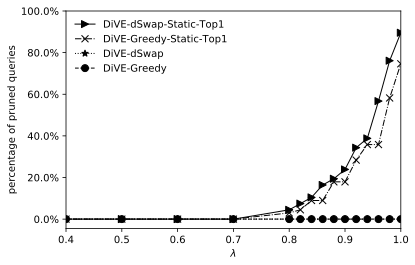
\includegraphics[width=4.0in]{figures/no_pruning_vs_static_extend}
		\vspace{-12pt}
		\caption{Static bound pruning performance while different value of $\lambda$, $k = 5$, MaxSum diversification function and running on Fligths dataset}
		\label{fig:static-pruning}
		\vspace{-20pt}
	\end{center}
\end{figure}

For the rest, we will use Top1 instead of MaxMin pruning due to we also have Swap technique that implement Top1 approach. The reason why we still need swap is because Greedy starts with small number of views in the initialization. Only two views as the set $ S $. Hence, while calculating the $ setDist $ of each views in $ X $, there are a lot of views have same score that it may decrease the chance of pruning. Moreover, there is no guarantee that two most distant views which selected by Greedy as the initialization have high importance score and there is no way to replace those two views. However, Swap has bigger number of views in the initialization (e.g. five views). While calculating the $ setDist $ of views in $ X $, the chance of views have same score is lower than Greedy. Additionally, swap also has a replacing mechanism that can replace low quality views in the current set with the better one. 


In this experiment, we used Flights dataset with 5 queries, Figure \ref{fig:static-pruning} shows top 1 algorithm which used Greedy and Swap techniques have similar performance.




\section{Distance Functions}


In terms of distance functions, I have been looking for the bounded distance function to compare between two probability distributions, there are several distance functions that I have studied: 

\begin{itemize}
	\item Euclidean distance, currently is used and the maximum bound is $ \sqrt{2} $.
	\item Kullback-Leiber (KL) distance, this distance is not bounded, the mathematically proof can be seen below.
	\item Earth Mover Distance (EMD), this distance is widely used and very good for comparing two probability distributions. Mostly this distance used in computer vision application to compare between two histograms. However, based on my finding, this distance is not bounded as well.
	\item Kolmogorov Distance has the maximum bound equal to 1. However, mostly example code that I found uses this distance as hypothesis test that need another parameters such as $\alpha$ and confidence interval. 
\end{itemize}
Until now, I am not sure if there is a bounded distance function that can be used for our work except the Euclidean distance. 

\subsection{Euclidean Maximum bound}
For the general case, Euclidean distance $d$ is defined as following: 
$d = \sqrt{\sum{(x-y)^2}}$, where $ \sum{(x-y)^2} = \sum x^2 + \sum y^2 - 2\sum xy$. Given that in probability vectors all values are nonnegative, $d$ is max when the last term is zero, then $d = \sum x^2 + \sum y^2$. All values are between 0 and 1 (sum up to 1), $\sum x = \sum y = 1$. The theoretical maximum is attained when $2\sum xy = 0$ and $\sqrt{2}$ as the maximum theoretical bound can be proven as following: 
\newline
$ \sqrt{\sum{(x-y)^2}} \leq \sqrt{\sum{(x)^2} + \sum{(y)^2}} $
\newline
$ \sqrt{\sum{(x-y)^2}} \leq \sqrt{1 + 1} $
\newline
$ \sqrt{\sum{(x-y)^2}} \leq \sqrt{2} $



%a2 + b2 = (a+b)2 - 2ab
%a2-b2 = (a-b)(a+b)
%(a+b)2 = a2+2ab +b2 
%(a-b)2 = a2-2ab +b2 
%(a+b+c)2 = a2 +b2 +c2 +2ab+2bc+2ac



\subsection{Maximum bound of Kullback-Leibler (KL) distance}

For distributions which do not have the same support, KL divergence is not bounded. Look at the definition: $KL(P\vert\vert Q) = \int_{-\infty}^{\infty} p(x)\ln\left(\frac{p(x)}{q(x)}\right) dx$

If $ P $ and $ Q $ have not the same support, there exists some point $x'$ where $p(x') \neq 0$ and $q(x') = 0$, making KL go to infinity. Even both distributions have the same support, when one distribution has a much fatter tail than the other. Then:
$$KL(P\vert\vert Q) = \int p(x)\log\left(\frac{p(x)}{q(x)}\right) \,\text{d}x$$
when
$$p(x)=\overbrace{\frac{1}{\pi}\,\frac{1}{1+x^2}}^\text{Cauchy density}\qquad q(x)=\overbrace{\frac{1}{\sqrt{2\pi}}\,\exp\{-x^2/2\}}^\text{Normal density}$$
then
$$KL(P\vert\vert Q) = \int \frac{1}{\pi}\,\frac{1}{1+x^2} \log p(x) \,\text{d}x + \int \frac{1}{\pi}\,\frac{1}{1+x^2} [\log(2\pi)/2+x^2/2]\,\text{d}x$$
and
$$\int \frac{1}{\pi}\,\frac{1}{1+x^2} x^2/2\,\text{d}x=+\infty$$

In conclusion, Kullback-Leibler (KL) is not bounded. For instance, when I implement KL in my code. In some case while the bin does not has its pair in the reference (which means 0), the result are two posibilities: error devided by 0 or $ log\ 0 $ which is undefined. 
\newline

\section{Max-sum and Max-min diversification}
Current results that we have are using MaxSum diversification. Based on my hypothesis and experiments that MaxMin Diversification can improve the pruning performance. The results while using MaxSum vs. MaxMin on Greedy Static Top1 and Swap Static Top 1 can be seen in Figure \ref{fig:maxsum-maxmin-greedy-swap}.

\begin{figure}
	\begin{center}
		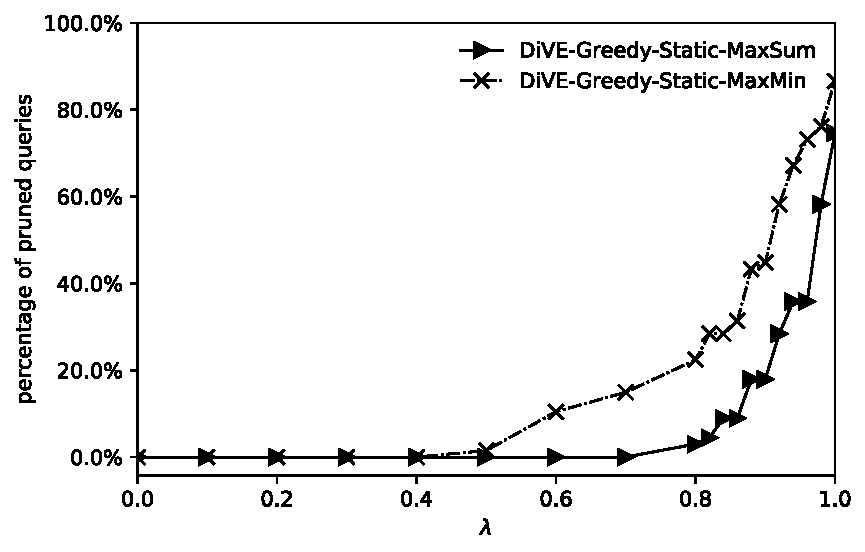
\includegraphics[width=3.0in]{figures/MaxSum_MaxMin_Greedy}
		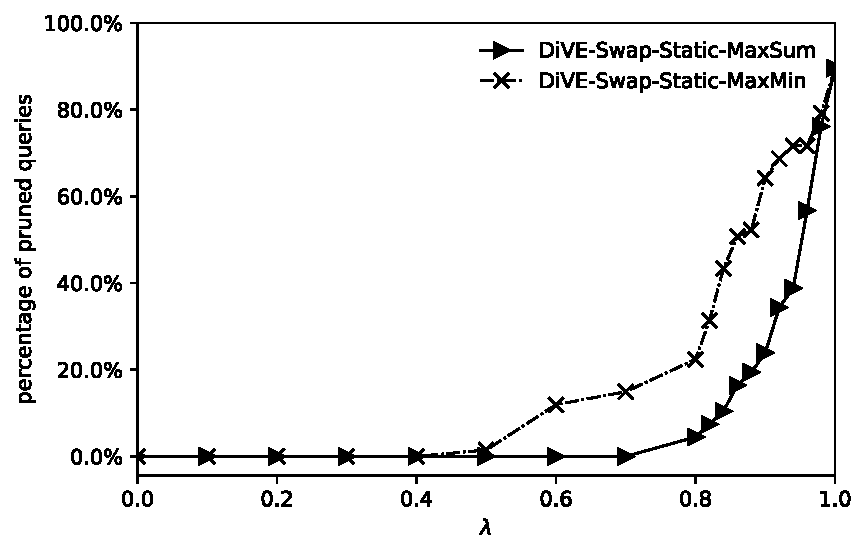
\includegraphics[width=3.0in]{figures/MaxSum_MaxMin_Swap}
		\caption{MaxSum vs. MaxMin diversification on Greedy and Swap running on Flights dataset, $k = 5$}
		\label{fig:maxsum-maxmin-greedy-swap}
	\end{center}
\end{figure}


MaxSum uses average score of diversity of the set $ S $ which is by computing the total sum of all distances then dividing by $ k*(k-1) $ while MaxMin uses the maximum of minimum score of distance in the set $ S $.  Hence, the range diversity score from those both approaches are different. For instance, there are three views in set $ Z $ which each view is different with others. The maximum score of distance between two views is $ 1 $ and the minimum is $ 0 $. Using MaxSum method the diversity score of set $ Z $ will be $ (1+1+1)/(3*(3-1)) = 0.5 $ whereas diversity score of MaxMin is $ 1 $ because the minimum distance in the set $ Z $ is $ 1 $. 

\begin{table}
	\begin{center}
	\caption{Example setDist score}
	\label{tab:setDist-score}
	\begin{tabular}{ccl}
		\toprule
		$ v $ in $ X $ &MaxSum &MaxMin\\
		\midrule
		$ v_1 $ & 0.5 & 1.0\\
		$ v_2 $ & 0.472222222 & 0.833333333\\
		$ v_3 $ & 0.444444444 & 0.666666667\\
		$ v_4 $ & 0.4166666667 & 0.5\\
		$ v_5 $ & 0.3899999999 & 0.333333333\\
		$ v_6 $ & 0.3611111111 & 0.166666667\\
		$ v_7 $ & 0.3333333333 & 0.166666667\\
		\bottomrule
	\end{tabular}
	\end{center}
\end{table}

The example variance of $ setDist $ score using Flights dataset between MaxSum diversification and MaxMin diversification can be seen in the Table \ref{tab:setDist-score}. In this experiment, I selected two most distant views as the initial set $ S $ and then calculate the $ setDist $ of all views in $ X $. For instance, the highest score of $ setDist $ is $ v1 $, where on MaxSum the maximum sore is $ 0.5 $ and on MaxMin the maximum score is $ 1 $. This Table is just an example, in the real data there are many views have same score. In this Table, I only want to show the distributions of $ setDist $ score and the different range of $ setDist $ score between MaxSum and MaxMin. 

\begin{figure}
	\begin{center}
	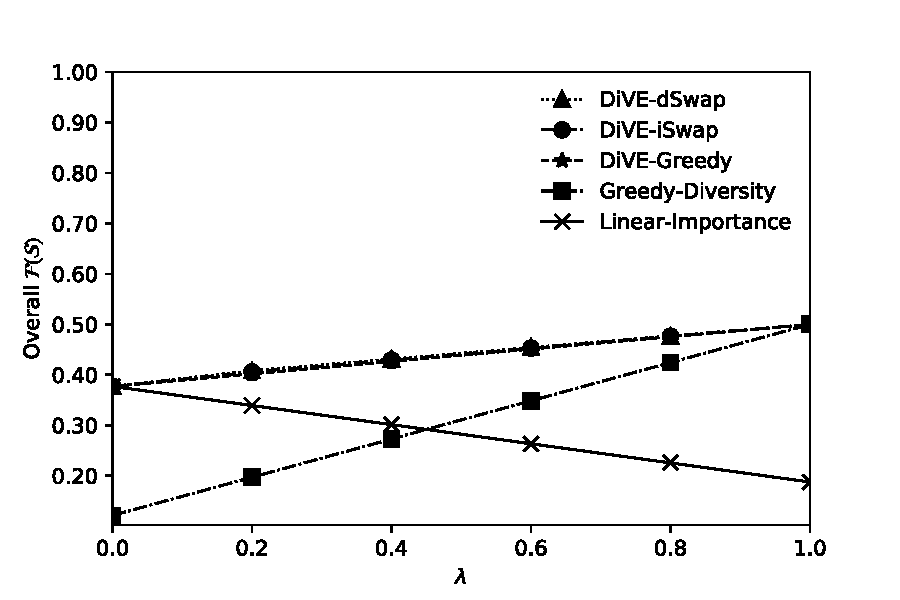
\includegraphics[width=3.0in]{figures/1_tradeoff_June_objf_disease_maxSUM}
	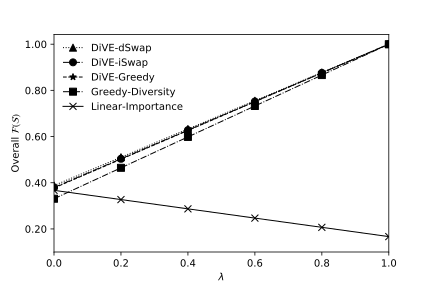
\includegraphics[width=3.0in]{figures/1_tradeoff_June_objf_disease_MaxMIN}
	\caption{Objective function shape on MaxSum vs. MaxMin diversification while different value of $\lambda$, $k = 5$}
	\label{fig:Objective-function-maxsum-maxmin}
	\end{center}
\end{figure}

Due to this different diversity score, MaxMin diversification can improve the pruning performance as shown in the Figure \ref{fig:Objective-function-maxsum-maxmin}, \textbf{in fact, I also found MaxMin diversification is able to start pruning while $\lambda = 0.4$ in some query subsets}. However, this MaxMin makes unbalance between the importance score and diversity score. The maximum diversity can be equal to $ 1 $ while the value of importance score is lower than that. This thing makes the shape of objective function unbalance. Please see Figure \ref{fig:Objective-function-maxsum-maxmin} below for more details.

\section{Total cost with and without pruning}
To see the performance of our proposed pruning approach, especially compared to schemes without pruning, Figure \ref{fig:flight_costs_all} shows the total cost running on Flights dataset. As shown in the Figure, DiVE-Greedy-Adaptive and DiVE-dSwap-Adaptive are able to reduce query cost. This experiment using adaptive algorithm while $ PI = 0.97 $ and this result is the avarage from five queries on Flights dataset. 

\begin{figure}
	\begin{center}
		\vspace{-50pt}
		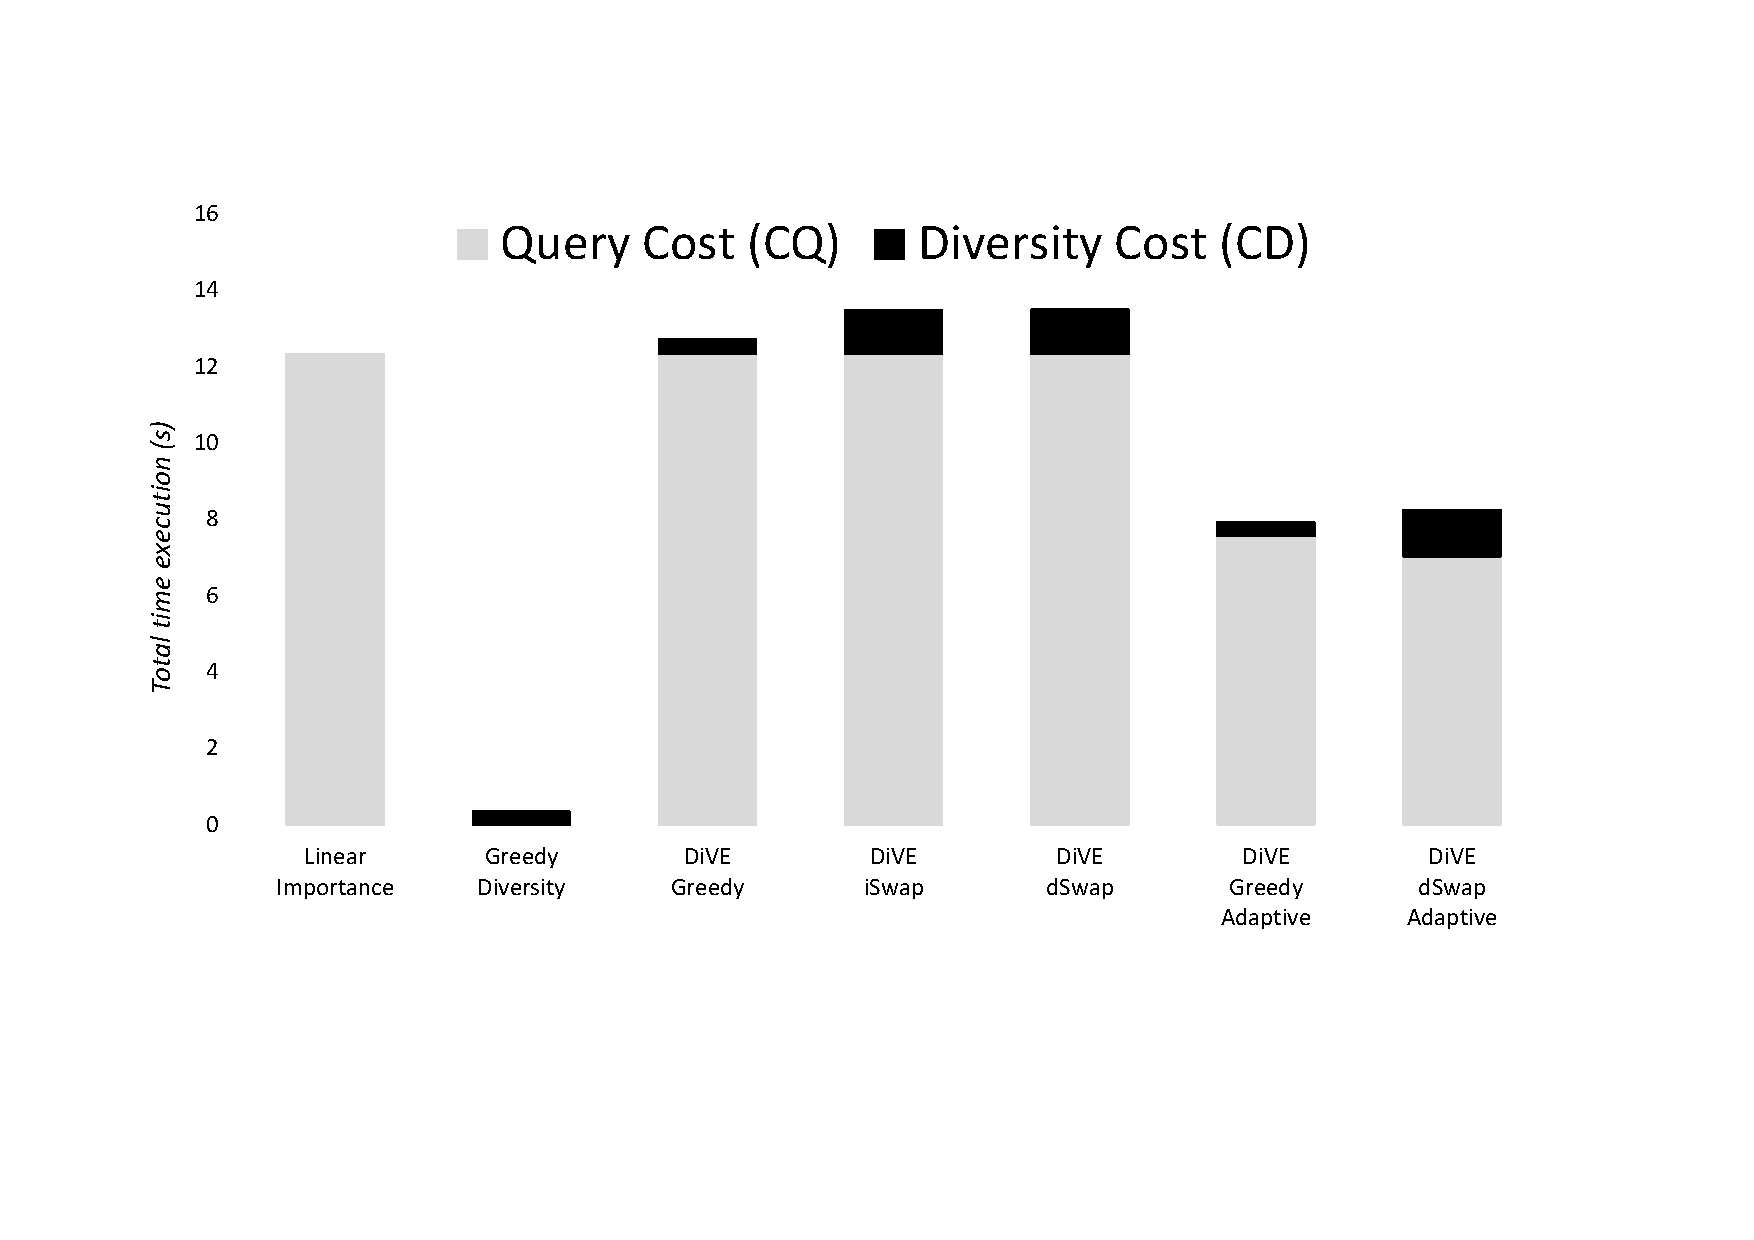
\includegraphics[width=7.0in]{figures/flight_costs_all}
		\vspace{-90pt}
		\caption{Total costs of schemes running on Flights dataset, MaxSum diversification, $k = 5$,  $ PI = 0.97 $, and $\lambda = 0.5$ }
		\label{fig:flight_costs_all}
		\vspace{-20pt}
	\end{center}
\end{figure}

\section{Impact of $ k $ to pruning performance}

Before observing the impact of $k$ to pruning performance, due to the Greedy algorithm has been changed which is using top1 approach, as the result, Greedy and Swap have close performance while using static bound as well as the adaptive bound. The performance of Greedy vs Swap while using static bound can be seen in the Figure \ref{fig:static-pruning} whereas the performance while using adaptive bound can be seen in the Figure \ref{fig:adaptive-pruning-performance}. Using adaptive maximum bound both DiVE-Greedy and DiVE-dSwap are able to prune queries start from $\lambda = 0.2$, and with higher $\lambda$ more queries are pruned. 

The next experiment is to observe the impact of $k$ to pruning performance while the $\lambda$ is constant. Figure \ref{fig:impact-of-k-pruning-performance} shows the impact of $k$ to pruning performance. This experiment running on Flights dataset, using 5 queries and $\lambda = 0.5$. The pruning performance is decreasing while $k$ is increasing. 

\begin{figure}
	\begin{center}
		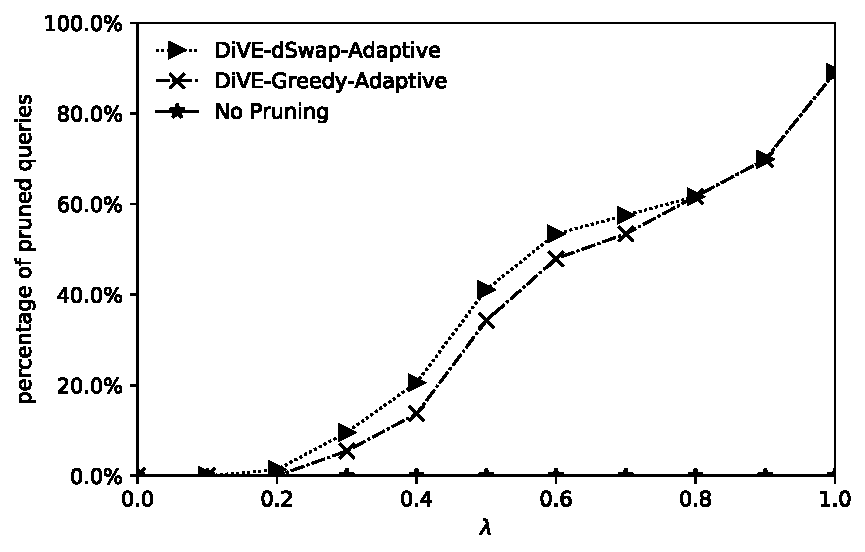
\includegraphics[width=4.0in]{figures/pruning_performance_greedy_dswap_adaptive}
		\vspace{-12pt}
		\caption{Adaptive bound pruning performance using different value of $ \lambda $, $k = 5$,  $ PI = 0.97 $, MaxSum diversification, running on Flights dataset}
		\label{fig:adaptive-pruning-performance}

	\end{center}
\end{figure}

\begin{figure}
	\begin{center}
		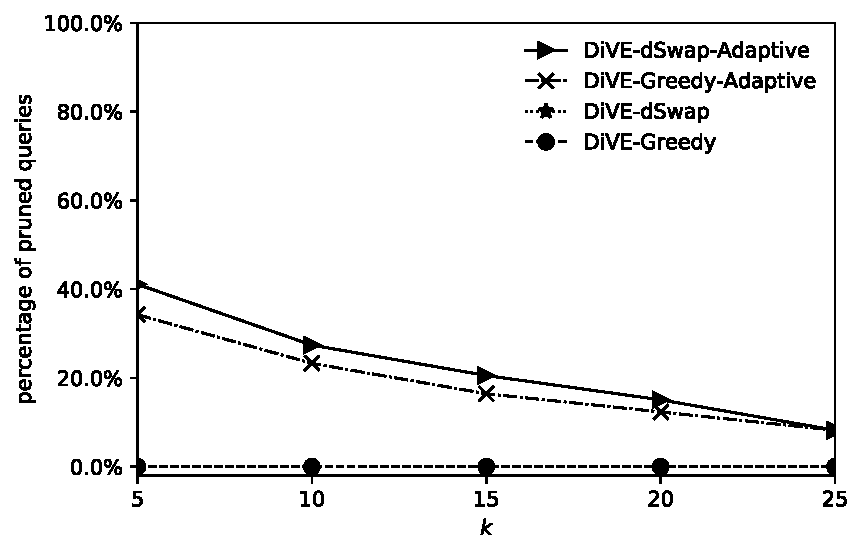
\includegraphics[width=4.0in]{figures/impact_of_k_to_pruning_adaptive}
		\vspace{-12pt}
		\caption{Impact of $k$ to pruning performance, $\lambda = 0.5$, MaxSum diversification, running on Flights dataset}
		\label{fig:impact-of-k-pruning-performance}
		
	\end{center}
\end{figure}


\section{DiVE-Greedy and DiVE-Swap complexity}
The costs of Greedy Construction algorithm has two components which are the query execution cost $C_Q$ that computing the importance score of view and the diversity cost $C_D$ that computing set distance of each view from the views already in S. The complexity of query execution cost is $ O$($n$) as the content of each view is generated only once. The diversity cost $C_D$ is $ O$($kn$) where $k$ is the size of subset of views $ S $ and $ n $ is the number of all possible views.


Meanwhile, The costs of Swap algorithm is also depend on the query execution time $C_Q$ of all possible views and the diversity computation $C_D$. The query cost $C_Q$ is executed only once but the cost is high due to it needs I/O cost. However, the complexity of diversity computation $C_D$ is $ O\left(k^2n \right) $ and the number of distance computation depends on the number of iterations of the swap and the number of views in $X$. In the worst case, swap algorithm can perform $ O\left(k^n \right) $. 

The different of total cost between Greedy and Swap approach can be seen in Figure \ref{fig:flight_costs_all}. Meanwhile, the impact of $k$ to the distance computation time while running on Flights dataset can bee seen in Figure \ref{fig:impact-of-k-diversity-computation}.

\begin{figure}
	\begin{center}
		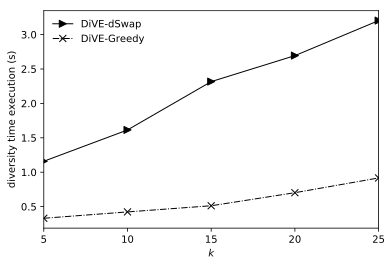
\includegraphics[width=4.0in]{figures/impact_of_k_to_diversity_cost}
		\vspace{-12pt}
		\caption{Impact of $k$ to diversity computation running on Flights dataset}
		\label{fig:impact-of-k-diversity-computation}
		
	\end{center}
\end{figure}

\section{Proposed algorithm's Figure}
We proposed DiVE scheme using two kinds of popular heuristic approach which are Greedy and Swap techniques. Figure \ref{fig:algorithm-figure} shows our proposed scheme technique. In case of Greedy, the set $ S $ is initialized by two most distant views. In each iteration, the best view in $ X $ that can maximize objective function $F(S)$ will be added to the set $ S $. Meanwhile, for the Swap case, the set $ S $ is initialized by the most diverse $  k $ views and in each iteration, all candidates views in $ X $ will be interchanged to set $ S $ and view which can improve the current objective function $F(S)$ will replace a view in set $ S $.

The $setDist$ score is used to sort all candidate views in $ X $, the highest score means that views is more diverse to set $ S $. The current bound is utilized to compute the estimate utility of each candidate view. First, the theoritical maximum bound ($ \sqrt{2} $) is used and this bound is updated while the actual importace score of view has been known. To avoid the wrong current bound, samping based on prediction interval is used. Before running the program, user needs to defined what PI that she wants to use. For instance, while users set PI to 80 then after 9 views is executed the current bound will be updated to the maximum bound which have seen so far. The most used PI can be defined as following: 

\begin{itemize}[noitemsep]
	\item PI80: need to execute 9 views
	\item PI85: need to execute 12 views
	\item PI90: need to executes 20 views
	\item PI95: need to executes 40 views
	\item PI97: need to executes 60 views
\end{itemize}


\begin{figure}
	\begin{center}
		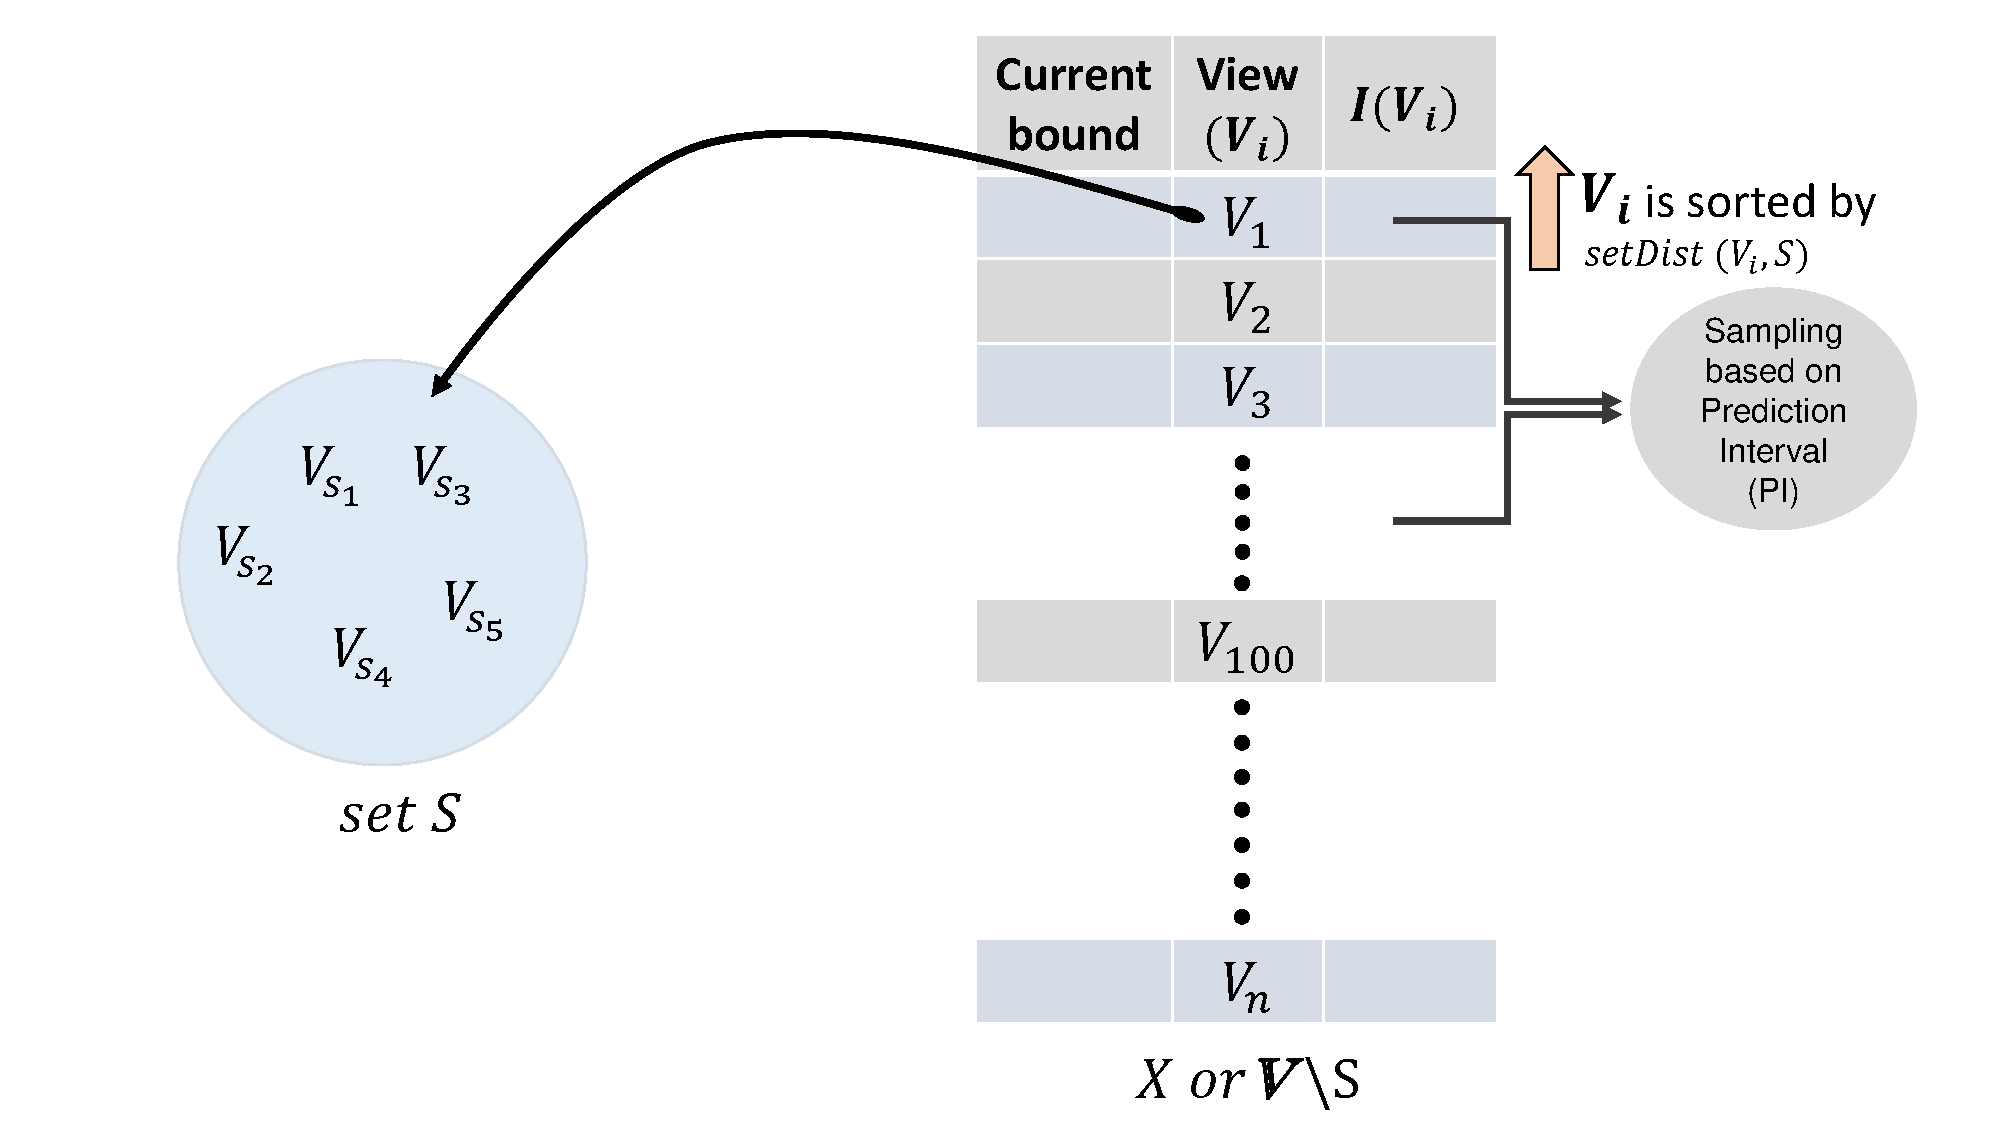
\includegraphics[width=5.0in]{figures/Algorithm}
		\vspace{-12pt}
		\caption{Utilizing $setDist$ score to sort candidate views and update current maximum bound to optimize the pruning performance}
		\label{fig:algorithm-figure}
		
	\end{center}
\end{figure}


\section{Query sharing computation}

Beside using pruning, SeeDB used query sharing optimizaation to reduce the query executions as well. To do query sharing optimization, SeeDB used combine multiple aggregates, combine multiple GROUP BY, and combine target and reference view query. However, pruning and query sharing seem two kinds of orthogonal optimizations. Hence, SeeDB proposed \textit{phased execution framework} which was by dividing dataset to phases. For instance, if we have 100,000 records in our dataset and we use 10 phases, the $i = 4^{th}$ processes records 30,001 - 40,000. 

In fact, SeeDB used partial result of each aggregate view on the fractions and used it to estimate the quality of each view and prune low-quality views in each phase. The query sharing optimization is used to minimize scans on the fraction of dataset in each phase whereas the pruning-based optimization is processed in the end of each phase.

If we see the SeeDB proposed approach, they divided the data to many phases and in the begining of phase, the query sharing computation is applied in the fraction and use that partial result to estimate the quality of view which still under consideration and in the end, the pruning-based optimizataion is applied. Due to of this, I do not think that this query sharing approach is applicable to our work. 

In case of our work, we sorted the remaining views based on $setDist$ score and execute the query view one by one start from the top and we need to know the importance score of executed view in order to get the current $ F(S) $ and to update the maximum bound. We also assume that by sorting the views based on $setDist$ the chance view is similar to others view in the above and below position are low. It means that to do query sharing execution by combining multiple aggregate or GROUP BY is difficult. There is no possibility to collect all views with same aggregate function or GROUP BY then execute in the same time due to we need to know the importance score of each view one by one.     

\section{Correcting wrong maximum bound in adaptive pruning scheme}
I developed a program that able to store all bound changed and pruned views in each bound changed. This program is not correcting the bound and bring back pruned views directly while the program realizes that the maximum bound is wrong. That is because while that approach is used, the program may face never ending looping because it repeats the previous wrong step while the maximum bound is wrong. The worst case happens while the view which has the maximum bound is in the below position of list $ X $, if the direct fixing approach is applied then the program always repeat previous step which has wrong maximum bound. 

In order to overcome this issue, this program runs until the end without caring the wrong maximum bound. Then, instead of showing the result to the user in the end of running, this program will re-run using the maximum bound that is founded in the first run which definitly the correct maximum bound. However, this approach seems running the program twice and it makes double execution time. 

\section{New Datasets}
- Not yet

\end{document}



%For the general case, Euclidean distance $d$ is defined as following: 
%$d = \sum{(x-y)^2} = \sum x^2 + \sum y^2 - 2\sum xy$. Given that in probability vectors all values are nonnegative, $d$ is max when the last term is zero, then $d = \sum x^2 + \sum y^2$.
%
%All values are between 0 and 1 (sum up to 1), $\sum x = \sum y = 1$. In such a vector, its theoretical maximum is attained when all its entries are 0 except one which is 1, it is when $\sum x^2 = \sum x$ and $\sum y^2 = \sum y$. It also follows from the above description, that then $\sum xy$ can very easily happen to be zero (since in each vector there is just single nonzero element).
%\newline

%Example maximum condition for two bins case: 
%\newline
%
%$\sum a = \sum b = 1$, $a , b \geq 0$
%\newline
%
%$(\sum a)^2 + (\sum b)^2 \geq \sum a^2 + \sum b^2$
%\newline
%
%$(\sum a)^2 + (\sum b)^2 \geq \sum a^2 + \sum b^2 - \sum 2ab $ 
%\newline
%
%$(\sum a)^2 + (\sum b)^2 \geq \sum (a^2 +  b^2 -  2ab)  $ 
%\newline
%
%$(\sum a)^2 + (\sum b)^2 \geq \sum (a-b)^2  $ 
%\newline
%
%$1 + 1 \geq \sum (a-b)^2  $ 
%\newline
%
%$\sqrt{2} \geq \sqrt{\sum (a-b)^2}  $ 
%\newline

%Max-sum is bi-criteria objective function to maximize the sum of the relevance and dissimilarity of the selected set, which can be defined as follows:
%
%\begin{equation}
%F\left(S\right) =  \left(1-\lambda\right) * I\left(S\right) + \lambda * f\left(S,D\right)
%\label{objectif_function}
%\end{equation}
%
%Where, 
%$ I\left(S\right)= \sum_{i=1}^{k} \dfrac{I(V_i )}{I_u}, V_i  \in S $ and $ f\left(S,D\right)= \dfrac{1}{k\left(k-1\right)}  \sum_{i=1}^{k} \sum_{j>i}^{k} D\left(V_i,V_j\right) ,V_i,V_j  \in S $
%\newline
%
%Meanwhile, Max-min diversification is the bi-criteria objective function that maximize the \textit{minimum} relevance and dissimilarity of the selected set. Based on the work of Gollapudi (An axiometic approach for result diversificaiton), this objective function can be defined as follows: 
%
%\begin{equation}
%F\left(S\right) = (1-\lambda) * \underset{u \in S} {\mathrm{min}} \ w\left(u\right)  + \lambda * \underset{u,v \in S} {\mathrm{min}} d\left(u,v\right)
%\end{equation}
%
%While Max-min diversification is to maximize the minimum of importance score, I am not sure this approach is relevant or not for our work. 